\chapter{Protoyp}
\section{Übersicht}
Der Tresh-Prototyp besteht aus einem Libelium Waspmote als \gls{iotk}, einem Raspberry Pi 3 als \gls{iotg} und \gls{siot} als \gls{iotp}.
\begin{figure}[H]
     \centering
        \includegraphics[width=1.0\textwidth]{pictures/PrototypeConcept.png}
    \caption{Gesamt-Architektur des Prototyps inklusive Schnittstellen}
    \label{fig:PrototypeConcept}
\end{figure}
Die Entwicklung des Prototyps bestand aus drei Teilen. Der Erste Teil war evaluation von geeigneter Hardware für den \gls{iotk} und den \gls{iotg}. Als nächstes musste die Hardware zusammengebaut werden, wobei hier ein massgeschneidertes Gehäuse per 3D-Druck entwickelt wurde. Parallel zur Entwicklung der Hardware wurde die Software für den Raspberry Pi und den Waspmote entwickelt. 

\section{Hardware}

\subsection*{\gls{iotk}-Evaluation}
Für die Evaluation des Knoten wurden verschiedene Embedded-Plattformen in Betracht gezogen. Da dies noch vor der definitiven Entscheidung für LoRa geschah, sind bei den Plattformen auch andere Funktechnologien berücksichtigt worden.

\subsubsection*{Sming}
Sming basiert auf dem TWX51-Sensor Node, welcher von Daniel Meer an der BFH/TI  entwickelt wurde. Herr Meer beschreibt den TWX51 wie folgt: 
\begin{quote}
\textit{Der TXW51 ist ein kleiner und energiesparender Sensorknoten, der als Basis für zukünftige Projekte verwendet werden
kann. Er kommuniziert über Bluetooth Smart und enthält einen Sensor zur Messung der Beschleunigung. Die Firmware kann einfach für neue Anforderungen modifiziert werden.}\autocite{bfh:TXW51}
\end{quote}

\begin{figure}[H]
     \centering
        \includegraphics[scale=0.6]{pictures/Sming.png}
    \caption{Sming mit Akku bestückt}
    \label{fig:Sming}
\end{figure}

\textbf{Vorteile}
\begin{itemize}
\item Eigenentwicklung der BFH/TI, Wissen komplett inhouse vorhanden
\item Optimiert für tiefen Energieverbrauch
\item sehr kleine Grösse (2.5cm x 1.7cm)
\item hat integrierte \gls{ble}-Schnittstelle
\end{itemize}
\textbf{Nachteile}
\begin{itemize}
\item kann zwar über Interrupts aufgeweckt werde, hat jedoch kein RTC
\item hat nur 3V-Spannung (nicht 3.3V), dadurch inkompatibel zu 5V-Sensoren
\item nur kurze Funk-Distanzen aufgrund von BLE
\item keine Lang-Distanz-Funk-Technik
\end{itemize}

\newpage

\subsubsection*{Tiny-Mesh}
Tiny-Mesh ist das Produkt des gleichnamigen Unternehmens aus Norwegen. Die Idee hinter diesm Produkt ist ein selbst-formendes und selbst-heilendes Sensor-Mesh-Netzwerk zu konstruieren, welches die Sensordaten der einzelnen Knoten an eine Cloud anbindet. Die Knoten basieren auf Modulen von Radiocraft, welche den proprietären Tiny-Mesh-Ptrotokoll-Stack implementieren. Für die Evaluation erhielten wir ein Starter-Kit zum testen.

\begin{figure}[H]
     \centering
        \includegraphics[scale=0.5]{pictures/TinyMesh.png}
    \caption{Radiocraft-Modul und die Batteriehalterung auf der Unterseite}
    \label{fig:TinyMesh}
\end{figure}

\textbf{Vorteile}
\begin{itemize}
\item Mesh-Netzwerk ermöglicht Erweiterung durch nodes
\item Mesh-Netzwerk ist selbst-heilend
\item Mesh-Netzwerk ist selbstkonfigurierend
\end{itemize}
\textbf{Nachteile}
\begin{itemize}
\item Proprietärer TinyMesh-Protokoll-Stack
\item Module sind nicht Programmierbar, Logik muss von externem Plattform gemacht werden
\item hoher Energieverbrauch durch Mesh-Topologie
\end{itemize}

\newpage

\subsubsection*{Waspmote}
Waspmote ist eine Mikrocontroller-Plattform von der Spanischen Firma Libelium. Die Plattform ist Modular aufgebaut und unterstützt verschiedenste Funktechniken wie Zigbee, GSM und unter anderem auch LoRa. Durch das modulare Design können Funkchips schnell ausgewechselt werden. Die Plattform ist praktisch um Prototypen zu erstellen, wird von Libelium aber auch als Produkt in Kombination mit über 100 verschiedenen Sensoren vertrieben.
\begin{figure}[H]
     \centering
        \includegraphics[scale=1.0]{pictures/Waspmote.png}
    \caption{Libelium Waspmote}
    \label{fig:Waspmote}
\end{figure}

\textbf{Vorteile}
\begin{itemize}
\item Modular aufgebaut und ideal für einen Prototyp
\item unterstützt viele Funk-Technologien
\item hat einen RTC und kann den Mikrocontroller deaktivieren um Energieverbrauch zu minimieren. (0.6µA Verbrauch wenn nur RTC in Betrieb)
\item viele GPIOs 
\end{itemize}
\textbf{Nachteile}
\begin{itemize}
\item relativ gross (7.3cm x 5.1cm)
\item teuer (allein ein Waspmote kostet 163 Euro, stand 24.06.2016)
\item verhältnismässig hoher Energieverbrauch, wenn in Betrieb (15mA) und nicht in sleep. Die Ursache davon sind jedoch die vielen GPIos was gleichzeitig ein Vorteil ist
\end{itemize}

\subsection*{Entscheidung}
Mit der Entscheidung, das Netzwerk auf LoRa aufzusetzen, war die Entscheidung schon fast getroffen. Der Sming hätte zwar auch mit einem LoRa-Chip verbunden werden können, dies wäre jedoch ein Projekt für Studenten der Elektrotechnik. Das Waspmote überzeugt mit seiner Modularität, dem vorhandensein eines RTCs und nicht zuletzt auch damit, dass die Plattform auch schon von Roger Jaggi und Pascal Bohni erfolgreich eingesetzt wurde.

\subsection{Distanz-Sensor}
Wie in Kapitel \ref{chapter:devOfUseCase} beschrieben wird der Füllstand des Mülleimers durch Distanz mittels Ultraschall gemessen. Für diese Messung wird der Ultraschall-Sensor "HC-SR04" eingesetzt. Er hat einen Messbereich von 2 bis 500cm. Dieser Bereich beinhaltet alle Distanzen, welche in allen handelsüblichen Mülleimern gemessen werden können. Falls eine Version für Container erstellt werden sollte, müsste ein Sensor mit grösserem Messbereich verwendet werden. 
\begin{figure}[H]
     \centering
        \includegraphics[scale=0.3]{pictures/HC-SR04.png}
    \caption{Ultraschall-Sensor HC-SR04}
    \label{fig:HCSR04}
\end{figure}

\subsection{\gls{iotg}}
Als \gls{iotg} wurde ein Raspberry Pi 3 eingesetzt. Dieser kleine, flexible Einplatinencomputer bietet viele Schnittstellen an, lässt die Wahl zwischen verschiedenen Betriebssystemen und hat eine grosse Community. Für den Anwendungsfall des Tresh-Gateways sind die Netzwerkschnittstellen, um das Gateway mit dem Internet zu verbinden und die USB-Schnittstellen, um das Waspmote Gateway\footnote{Waspmote Gateway: \url{http://www.libelium.com/products/waspmote/interfaces/\#gateway_marker} Slide 11} an das Raspberry Pi anzuschliessen, essenziell. Das Raspberry Pi 3 bietet dazu zusätzlich zur Ethernet Schnittstelle auch gleich ein fest eingebautes \gls{wlan} Modul an, was viel flexibilität bei der Platzierung des Gateways ermöglicht. Nichtsdestotrotz ist natürlich die Ethernet-Schnittstelle zu bevorzugen, da diese eine stabilere Netzwerverbindung zur Verfügung stellt als die \gls{wlan} Schnittstelle. 

\section{Hardware-Implementation}
Nachdem die die Ware verfügbar war, wurde ein erster Proof-of-Concept aus Holz und einem grossen Breadboard erstellt. Dieser Prototyp hatte Hardwaremässig bereits die volle Funktion. Softwaremässig konnte er ganz rudimentär die gemessene Distanz via LoRa versenden.

\begin{figure}[H]
     \centering
        \includegraphics[scale=0.6]{pictures/Prototype1.jpg}
    \caption{Erster Prototyp des \gls{iotk}}
    \label{fig:HCSR04}
\end{figure}

Damit dieser Knoten jedoch in einem Mülleimer eingebaut werden kann, braucht er ein schützendes Gehäuse, damit er einerseitz nicht einfach verschmutzt und andereseits stabil im Eimer montiert werden kann. Mithilfe der Opensource-Software OpenSCAD konstruierten wir ein zweistöckiges Gehäuse. Im oberen Teil ist der Platz für das Waspmote und ein kleines Breadboard für den Ultraschall-Sensor, im unteren Stock ist Platz für die Batterie. Die Batterie ist ein 6600mAh-Akku, welcher von Libelium für das Waspmote angeboten wird. 
 
\begin{figure}[H]
     \centering
        \includegraphics[width=1.0\textwidth]{pictures/OpenSCAD.png}
    \caption{Entwicklung des Gehäuses für den Prototyp}
    \label{fig:OpenSCAD}
\end{figure}

Das Konzept des Gehäuses ist ein Schubladensystem. Das bedeutet, dass die Platine, welche die beiden Kammern des Gehäuses trennt, wie ein Schlitten in das Gehäuse einfahrbar ist. Auf dieser Platine wir auch Was Waspmote und der Sensor montiert. Dies hat zum Vorteil, dass bei einem Wartungszugriff die ganze Hardware einfach aus dem Gehäuse gezogen werden kann.
Das Gehäuse druckten wir auf einem Ultimaker 3D-Drucker aus. Es benötigte mehrere Testdrucks und verschiedenste Anpassungen am Plan bis das Gehäuse mit allen Komponenten zusammenpasste. Besonders delikat war das Schubladensystem, da der Schlitten mit 1mm Dicke nur gerade das zehnfache der Genauigkeit des 3D-Druckers ist.

\begin{figure}[H]
     \centering
        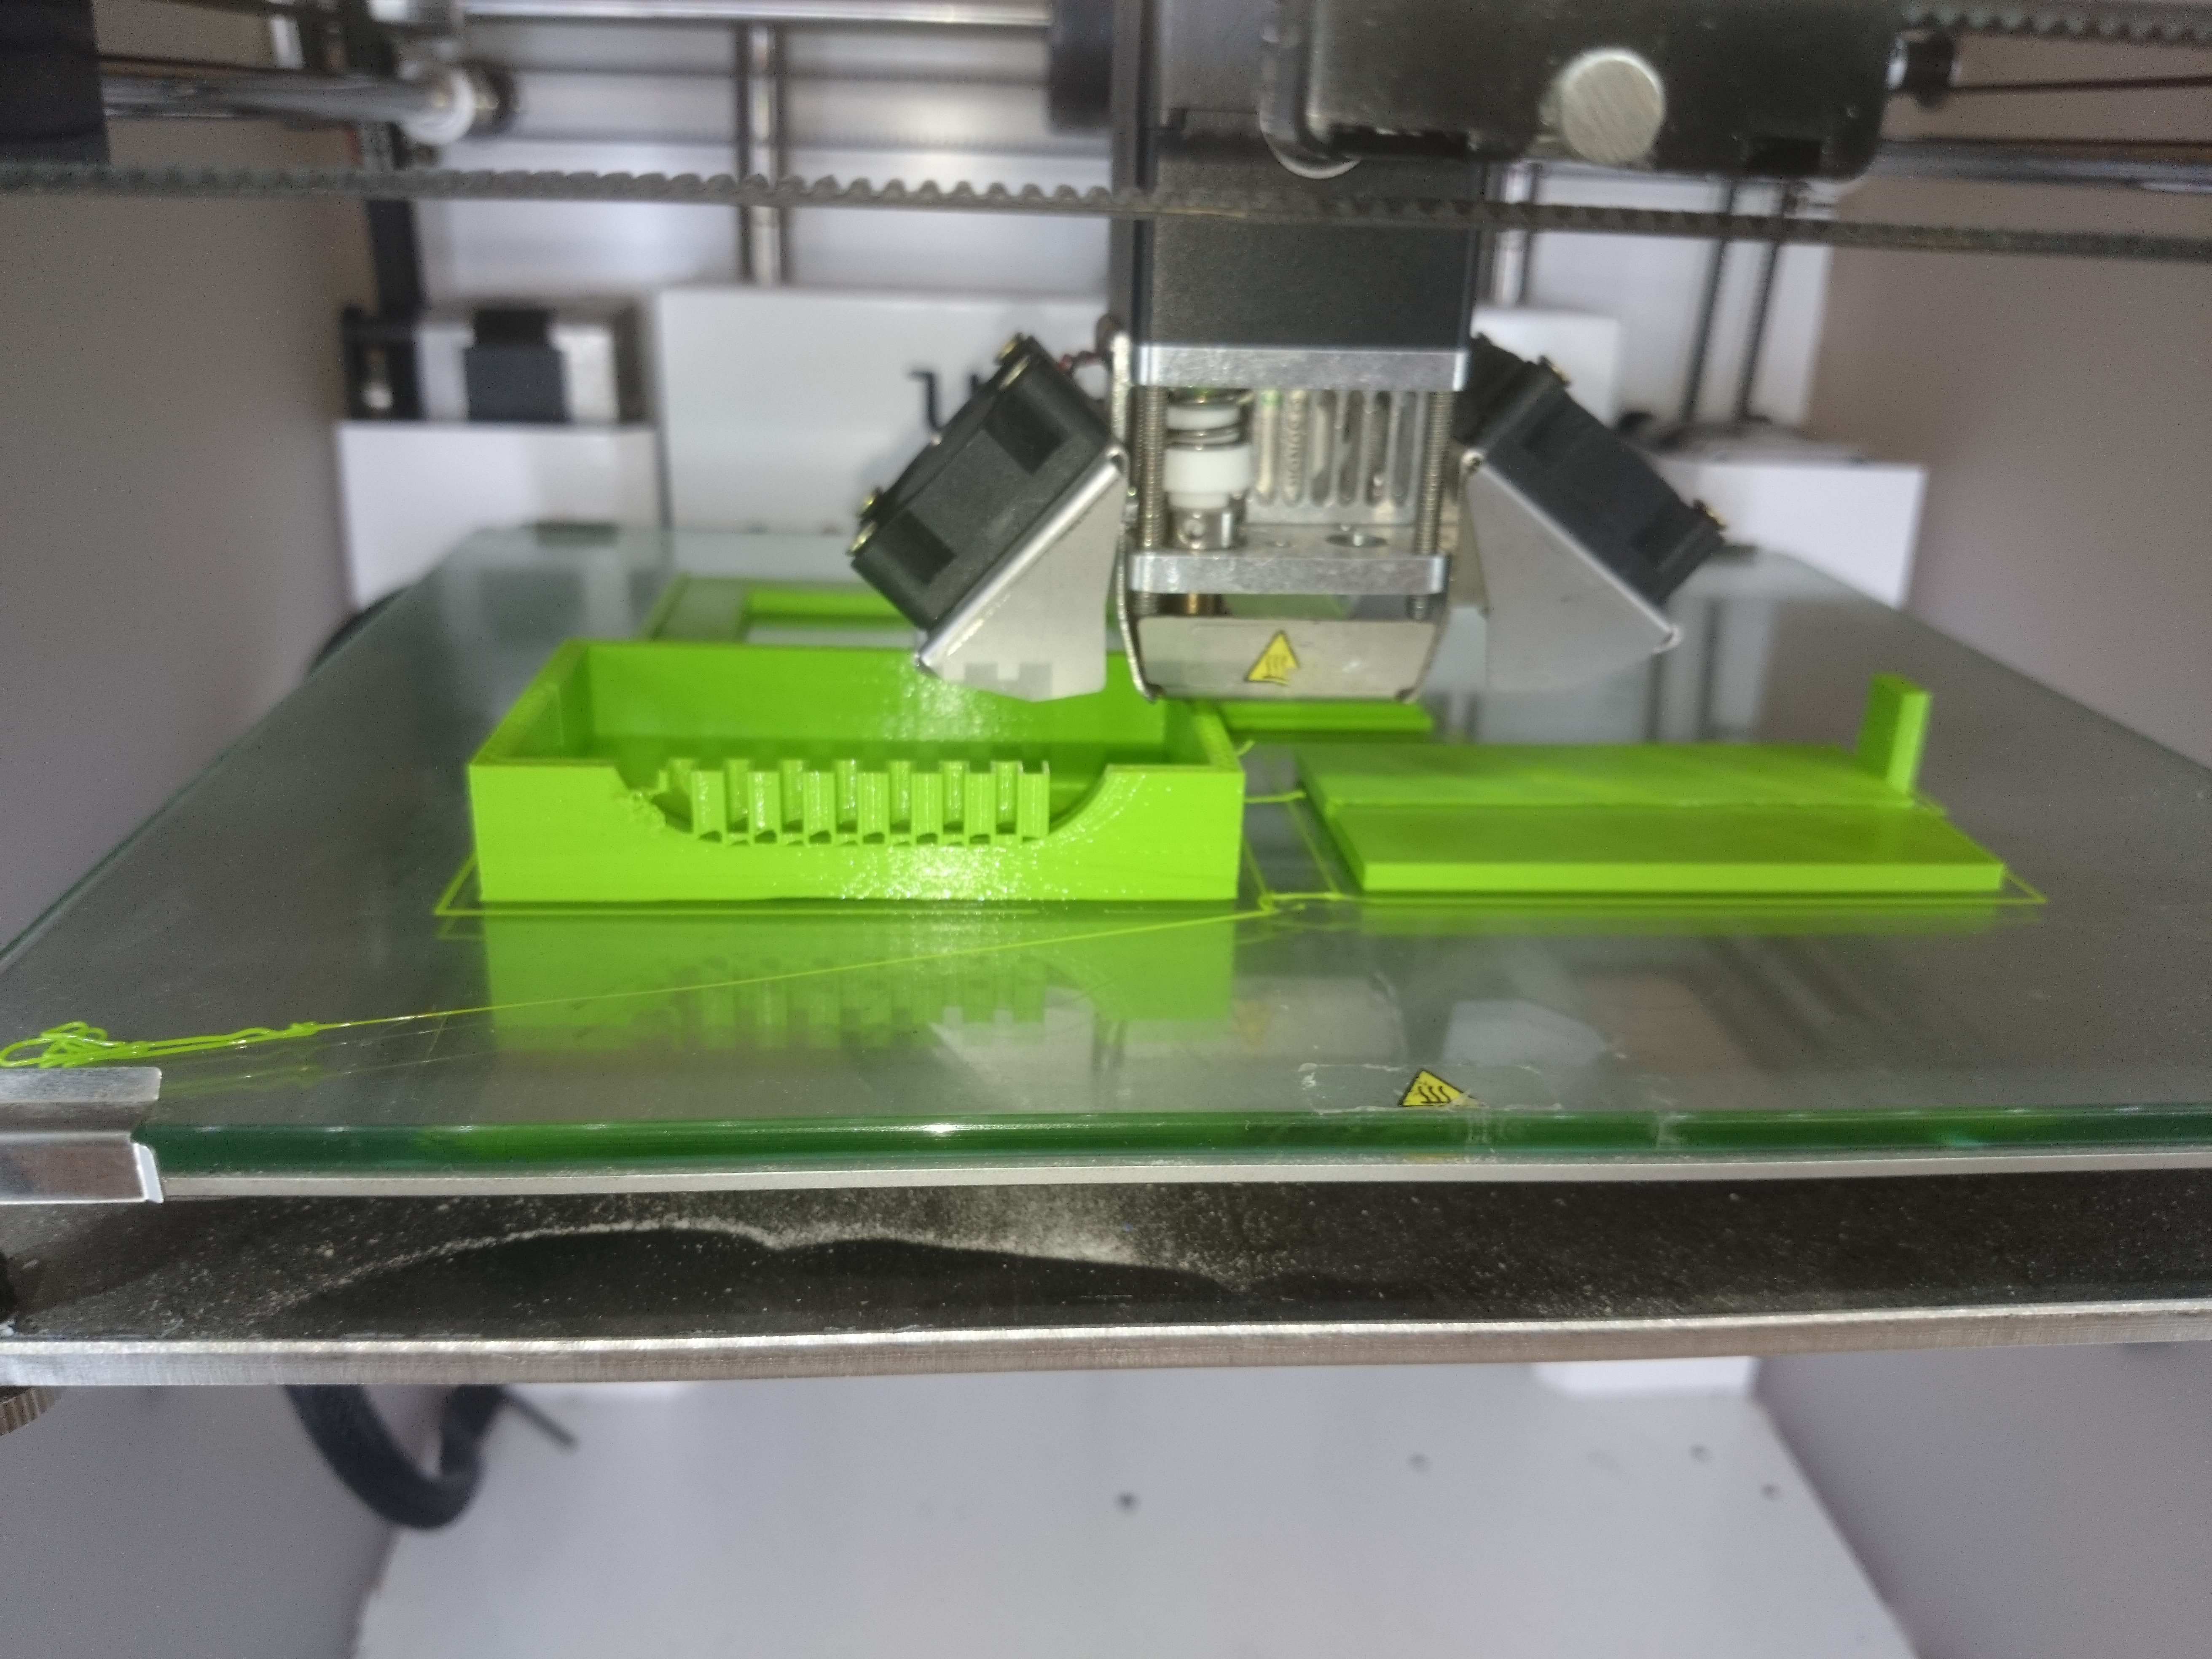
\includegraphics[width=0.55\textwidth]{pictures/3D-Print.jpg}
    \caption{Druck eines Gehäuse-Prototyps mit Ultimaker}
    \label{fig:3D-Print}
\end{figure}

Nachdem alle Gehäusekomponeten zusammenpassten und das Waspmote und das Breadboard montiert werden konnten, starteten wir die "Massenproduktion". Mit Massenproduktion ist in diesem Zusammenhang eine Stückzahl von 3 gemeint.

\begin{figure}[H]
     \centering
        \includegraphics[width=0.8\textwidth]{pictures/Massproduction.jpg}
    \caption{Die 3 fertigen Prototypen}
    \label{fig:3-Prototypes}
\end{figure}

Als nächstes mussten die Prototypen natürlich auch in den Einsatz gebracht werden. Als Testumfeld wurden zusammen mit Herr Danuser die PET-Eimer des Rolex-Gebäudes der BFH in Biel ausgewählt. Herr Danuser holte bei Herrn Schüpbach, dem Leiter des Hausdienstes, die Erlaubnis ein. Dieser erlaubte uns, im PET-Eimer in der Mensa und im PET-Eimer im 5. Stock des Gebäudes einen Sensor zu platzieren.

\subsection*{Installation}
Am Freitag, den 10. Juni 2016 konnten wir die Sensoren an ihren Standorten platzieren. Für den Raspberry Pi mit dem Waspmote-Gateway stellte uns Herr Danuser sein Büro zur Verfügung, damit dieser eine unversiegende Energiequelle sowie Ethernet-Anschluss hat.
Dabei mussten wir feststellen, dass definitiv der Spreizfaktor von LoRa benötigt wird, damit das Gateway den Sensor in der Mensa noch "hört". Der Sensor sendet mit 7dB Ausgangsleistung, das Gateway hat mit dem maximalen Spreizfaktor von LoRa eine Empfindlichkeit von -136dBM. Dies ergibt ein Powerbudget von 143dB, welches auch ziemlich ausgenutzt wird. Das Gateway sendet jeweils eine Ack-Bestätigung, wenn ein Sensor ein Packet versandt hat. Damit diese Ack-Packete garantiert ankommen, sendet das Gateway mit 14dB.

\begin{figure}[H]
     \centering
        \includegraphics[width=0.7\textwidth]{pictures/Tresh-Deployed.jpg}
    \caption{Der am aufgeklappten Deckel des PET-Eimers in der Mensa befestigte Prototyp}
    \label{fig:3-Prototypes}
\end{figure}

Der zweite Sensor im 5. Stock konnte leider nicht installiert werden. Der dortige Eimer ist komplett aus Metall konstruiert. Sobald der Sensor im Eimer eingeschlossen ist, wird sein Signal durch Reflexionen und Dämpfung des Eimers um ungefähr 45dB gedämpft. Das restliche Powerbudget von 98dB reicht leider nicht aus um das Gateway in Herrn Danuser's Büro zu erreichen. Der Prototyp bräuchte ein Koaxialkabel, damit wir seine Antenne ausserhalb des Eimers befestigt werden könnte und nur durch das Koaxial-Kabel zum Prototypen im Eimer verbunden wäre.


\section{Software}

\subsection{Waspmote als \gls{iotk}}


\subsection{Raspberry Pi als \gls{iotg}}

Die Hauptfunktion eines \gls{iotg} ist es ein Sensor Netzwerk mit einer \gls{iotp} zu verbinden. Genau diese Funktion wurde auf dem Raspberry Pi durch zwei Softwarekomponenten implementiert:

\begin{enumerate}
	\item tresh-lora-gateway - Sensordaten aus dem \gls{lora}-Netzwerk auf dem Waspmote Gateway empfangen.
    \item tresh-siot-gatway - Sensordaten des Waspmote Gateway an die \gls{siot} \gls{iotp} senden.
\end{enumerate}

Der dazugehörige Quellcode ist im Anhang unter \ref{appendix:raspberrypi} aufgeführt.

\subsubsection*{tresh-lora-gateway}

Die Aufgabe dieser Softwarekomponente ist es die Sensordaten aus dem \gls{lora}-Netzwerk zu empfangen und über USB eine serielle Schnittstelle zu emulieren welche die Daten ausgibt.

\subsubsection*{tresh-siot-gatway}

Die Aufgabe dieser Softwarekomponente ist es die Sensordaten über die serielle Schnittstelle zu empfangen und über \gls{mqtt} an die \gls{siot} \gls{iotp} weiterzuleiten. In der Bachelor Thesis \autocite{bfh:optimizedDataTransmission} hat Roger Jaggi die \gls{nodejs}-Applikation siot.net-nodejs-api\autocite{bfh:siot.net-nodejs-api} geschrieben, welche die \gls{siot} Gateway API Spezifikation implementiert. Die tresh-siot-gatway Applikation baut auf dieser API auf. Wir haben zusätzlich das Auswählen und Auslesen des seriellen Ports und die Zuweisung der empfangenen Sensordaten an die entsprechenden, in \gls{siot} registrierten Sensoren implementiert. Diese Zuweisung geschieht aktuell lokal auf dem \gls{iotg} anhand der \gls{lora} Netzwerk Adresse der \gls{iotk}. In Zukunft sollte diese Zuweisung aber auf einer höheren Sofwareschicht implementiert werden.

\subsection{\gls{siot}}
